\documentclass[border=5pt]{standalone}
\usepackage{tikz}
\usetikzlibrary{calc, positioning}
\usepackage{amsmath}
\begin{document}
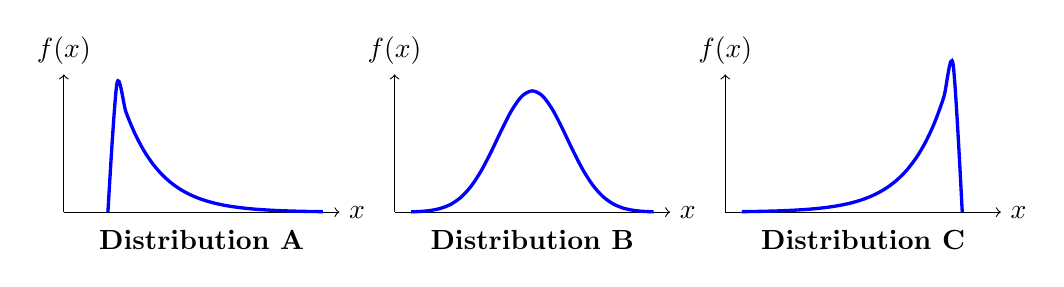
\begin{tikzpicture}[scale=0.7]
% Distribution A - Right skewed
\begin{scope}[xshift=0cm]
\draw[->] (0,0) -- (5,0) node[right] {$x$};
\draw[->] (0,0) -- (0,2.5) node[above] {$f(x)$};
\draw[blue, very thick] plot[smooth, domain=0.8:4.7] (\x, {2.2*exp(-1.5*(\x-1))*(\x > 0.8 ? 1 : 0)});
\node at (2.5,-0.5) {\textbf{Distribution A}};
\end{scope}

% Distribution B - Symmetric
\begin{scope}[xshift=6cm]
\draw[->] (0,0) -- (5,0) node[right] {$x$};
\draw[->] (0,0) -- (0,2.5) node[above] {$f(x)$};
\draw[blue, very thick] plot[smooth, domain=0.3:4.7] (\x, {2.2*exp(-(\x-2.5)^2/0.8)});
\node at (2.5,-0.5) {\textbf{Distribution B}};
\end{scope}

% Distribution C - Left skewed
\begin{scope}[xshift=12cm]
\draw[->] (0,0) -- (5,0) node[right] {$x$};
\draw[->] (0,0) -- (0,2.5) node[above] {$f(x)$};
\draw[blue, very thick] plot[smooth, domain=0.3:4.3] (\x, {2.2*exp(-1.5*(4-\x))*(\x < 4.2 ? 1 : 0)});
\node at (2.5,-0.5) {\textbf{Distribution C}};
\end{scope}
\end{tikzpicture}
\end{document}
